\documentclass[dvipsnames]{beamer}

\usepackage{preamble}
\usepackage{coursespecific}
\renewcommand*{\IncludeAnswers}{1}

\renewcommand*{\Lecture}{3}
\subtitle{Database Driven Web-applications}


\begin{document}

\begin{frame}
  \titlepage{}
\end{frame}

\begin{frame}
  \frametitle{Ingredients For Web-applications}
  
  \begin{itemize}
  \item User-interface in HTML and CSS
  \item Data in SQL database
  \item Business-logic in Python
  \end{itemize}

\end{frame}


\begin{frame}
\frametitle{Server-Side Web Scripting---A Three-tier Architecture}

\begin{center}
  \begin{tikzpicture}[thick,>=stealth]
    \small
    \fill[blue!25] (-1.5,.6) rectangle (5.5,1.8);
    \path 
    (-4.5,1.2) node[draw,ellipse,minimum size=10mm](Client) {Client}
    (0,1.2) node[draw,rectangle,minimum size=10mm,fill=white](WS) {Web Server}
    (4,1.2) node[draw,rectangle,,minimum size=10mm,fill=white](DB) {Database Server}
    ;
    \draw[<-] (Client.north east) -- node[fill=white]{1} (WS.north west);
    \uncover<2->{\draw[->] (Client) -- node[fill=white]{2} (WS);}
    \uncover<3->{\draw[<->] (WS) -- node[fill=blue!25]{3} (DB);}
    \uncover<4->{\draw[->] (WS.south west) -- node[fill=white]{4} (Client.south east);}

  \end{tikzpicture}
\end{center}


\begin{enumerate}
\item A client obtains an HTML page with an HTML form from a Web server.
\item<2-> The client completes the HTML form, and sends it back to the
  Web server.
\item<3-> The Web server executes a program that processes data from
  the client, for instance by updating a database.
\item<4-> The Web server sends an HTML page back to the client.
\end{enumerate}

% If the HTML code is simple and does not contain too much JavaScript,
% the page can be shown by most browsers.

% The HTML code is normally presented quickly by the browser, but the
% user interface is not like a normal desktop program.
\end{frame}



\begin{frame}
\frametitle{Why Should You Care About Learning HTML?}

\begin{itemize}
  
\item To be certain that a Web site works with all browsers
  
\item There are things that cannot be done with a WYSIWYG HTML editor
  
\item To reuse HTML code written by others
  
\item WYSIAYG = What You See Is All You Get; sometimes HTML editors
  generate unnecessary HTML
  
\item For Web programming, one writes programs that \emph{generate}
  HTML; so Web programming requires that one understands HTML

\end{itemize}
\end{frame}


% \begin{frame}
%   \frametitle{Why Use An HTML Editor?}

%   Why use a HTML editor like Microsoft Frontpage, DreamWeaver, or Nvu rather
%   than writing the HTML by hand?

%   \begin{uncoverenv}<2->
%     \begin{itemize}
%     \item It always generate correct HTML (or so it should)
%     \item One can learn HTML from it (but be aware of browser specific
%       code)
%     \item It is easier to get going
%     \end{itemize}
%   \end{uncoverenv}
% \end{frame}


\begin{frame}[fragile]
\frametitle{HTML in 21 minutes}

A legal HTML document (\examplefile{legal.html}):

\begin{small}
\begin{verbatim}
<html>
  <head>
     <title>Ken's Page</title>
  </head>
  <body>
    <h2>Ken's Marvellous Home Page</h2>
      I teach at the
      <a href="http://www.ku.dk">
       University of Copenhagen
      </a>
  </body>
</html>
\end{verbatim}
\end{small}

\begin{itemize}
\item Try to format HTML code nicely and consistent

\item Write the HTML code yourself

\item Later we shall construct programs that generate HTML code
\end{itemize}

\end{frame}

\begin{frame}
\frametitle{General Page Layout}

You should know about the following tags in HTML:

\begin{itemize}
\item Headings: \texttt{<h1>}\ldots \texttt{</h1>}, \ldots, \texttt{<h4>}\ldots \texttt{</h4>}
\item Rules: \texttt{<hr />}
\item Paragraphs and line breaks: \texttt{<p>}\ldots \texttt{</p>},
  \texttt{<br />}
\item Quotes: \texttt{<blockquote>}\ldots \texttt{</blockquote>}
\item Centering: \texttt{<center>}\ldots \texttt{</center>}
\item Bold text: \texttt{<b>}\ldots \texttt{</b>}
\item Italic text: \texttt{<i>}\ldots \texttt{</i>}
\item Underlined text: \texttt{<u>}\ldots \texttt{</u>}
\item Ordered lists: \texttt{<ol>}\ldots \texttt{</ol>}
\item Unordered lists: \texttt{<ul>}\ldots \texttt{</ul>}
\item List items: \texttt{<li>}\ldots \texttt{</li>}
\end{itemize}
\end{frame}

\begin{frame}
\frametitle{Hyper Links, Tables, and Images}
\begin{itemize}
\item Hyper links: \texttt{<a href="link">name</a>}
\item Local \emph{named} hyper links: \texttt{<a
    name="thename">}\ldots\texttt{</a>}
\item References to a name: \texttt{<a href="index.html\#thename">The Name</a>}
\item Mail-to links: \texttt{<a href="mailto:kfl@itu.dk">kfl@itu.dk</a>}
\item Tables: \texttt{<table>}\ldots \texttt{</table>}, \texttt{<tr>}\ldots
  \texttt{</tr>}, \texttt{<th>}\ldots \texttt{</th>} and \texttt{<td>}\ldots
  \texttt{</td>}
\item Images: \texttt{<img src="pluto.jpg" />}
\item Colors: use Cascading Style Sheets (CSS)
\end{itemize}
\end{frame}

\begin{frame}[fragile]
\frametitle{HTML forms}
  
A form can contain text areas (\verb+<textarea>+),
input fields (\verb+<input>+), and menus (\verb+<select>+)

Example: \examplefile{formular.html}

\begin{verbatim}
   <form action="mailto:kflarsen@diku.dk" 
         method="post" enctype="text/plain">
     ... more code ...
     <input type="reset" value="Start Over!" />
     <input type="submit" value="Send Form" />
   </form>
\end{verbatim}

Attributes to the \verb+<form>+ tag \texttt{action}, \texttt{method}( ,
and sometimes \texttt{enctype}) are important.  But postpone their
treatment till later.

% \begin{itemize}
% \item \verb+action="mailto:kflarsen@diku.dk"+:\\ the completed form is sent
%   by email
  
% \item \verb+method="post"+ should be used when the completed form is
%   sent by email
  
% \item \verb+enctype="text/plain"+ sends the form as ordinary text
%   (not encoded)
% \end{itemize}

A click on \verb+<input type="submit" value="Send Form" />+ sends the
completed form.

A click on \verb+<input type="reset" value="Start Over" />+ resets all
fields, text areas, and menues.
\end{frame}

\begin{frame}[fragile]
\frametitle{Text Areas --- \texttt{<textarea>}}
  
  In a text area (\verb+<textarea>+) any text can be written:

\begin{verbatim}
   <textarea name="comments" rows="5" cols="80">
     Write your comments here!
   </textarea>
\end{verbatim}

The attributes:

\begin{itemize}
\item \verb+name+ specifies a name for the field

\item \verb+rows+ specifies the number of lines (rows) in the text area
  
\item \verb+cols+ specifies the number of characters (columns) in each
  line in the text area
\end{itemize}


\end{frame}

\begin{frame}[fragile]
\frametitle{Input Fields --- \texttt{<input>} Text and Passwords}
  
  The attribute \verb+type+ determines the type of the input field:

\begin{itemize}
\item Single-line text areas:\\
\verb+<input type="text" name="lastname" />+


\item Passwords, which are not to be displayed by the browser:\\
  \verb+<input type="password" name="studentid" />+
  
\end{itemize}
\end{frame}
 

\begin{frame}[fragile]
\frametitle{Input Fields --- \texttt{<input>} Check Boxes and Buttons }
  
  More \texttt{input} types:

\begin{itemize}
\item Check boxes, possibly more
  than one item can be checked at a time:
  \begin{small}
\begin{verbatim}
<input type="checkbox" name="paper" value="nytimes" /> 
<input type="checkbox" name="paper" value="wpost" />
<input type="checkbox" name="paper" value="guardian" />
\end{verbatim}  
  \end{small}

\item Radio buttons, only one item can be checked at a time:
  \begin{footnotesize}
\begin{verbatim}
<input type="radio" name="sex" value="male" />
<input type="radio" name="sex" value="female" checked="yes" />
\end{verbatim}
  \end{footnotesize}
\item Button for resetting a form:
  \begin{small}
\begin{verbatim}
<input type="reset" ... />
\end{verbatim}
  \end{small}
\item Button for sending a completed form:
  \begin{small}
\begin{verbatim}
<input type="submit" ... />
\end{verbatim}
  \end{small}
\end{itemize}
\end{frame}





\begin{frame}[fragile]
\frametitle{Menu Choices, \texttt{<select>}}

\begin{itemize}
\item A drop-down menu, which allows the user so choose between a
  series of items (+<option>+):
  \begin{small}
\begin{verbatim}
<select name="order">
  <option value="9">Pepperoni Pizza</option>
  <option value="70">Pizza Bambino</option>
  <option value="47">Chicken Dipper (9 pieces)</option>
</select>
\end{verbatim}
  \end{small}
\item The attribute \verb+multiple+ in the \verb+<select>+ tag allows
  the user to choose more than one item.
\end{itemize}


\textbf{Complete form}

\begin{itemize}
\item Bare, with no layout structure: \examplefile{formular.html}
\item An example course evaluation with a nicer lay-out (using
  \verb+<table>+): \examplefile{formular2.html}
\end{itemize}

\end{frame}

\begin{frame}[fragile]
\frametitle{Completed Questionnaire, When Sent By Email}

\textbf{With} \verb+enctype="text/plain"+:

\begin{small}
\begin{verbatim}
 lastname=Olsen
 studentid=da4567
 sex=male
 paper=guardian
 comments=This is not a nice questionnaire.
 order=9
\end{verbatim}
\end{small}


\textbf{Without} \verb+enctype="text/plain"+:

\begin{small}
\begin{verbatim}
 lastname=Olsen&studentid=da4567&sex=male&paper=guardian
 &comments=This+is+not+a+nice+questionnaire.&order=9
\end{verbatim}
\end{small}
\end{frame}

\begin{frame}[fragile]
\frametitle{Find five bugs}

In an HTML document without consistent indentation:
\begin{footnotesize}
\begin{verbatim}
  <html><head><title>Hello</title></head>Hello<center>great page<p>
  this is in <b>bold<i> and italics</html>
\end{verbatim}
\end{footnotesize}
\begin{uncoverenv}<2->
  In an HTML document with consistent indentation:
  \begin{footnotesize}
\begin{verbatim}
  <html>
    <head>
      <title>Hello</title>
    </head>
    Hello
    <center>
      great page
      <p>
      this is in <b>bold<i> and italics
  </html>
\end{verbatim}
   \end{footnotesize}
%   Firefox shows this document without errors! Or does it?
 \end{uncoverenv}
\end{frame}


\begin{frame}
  \frametitle{Cascading Style Sheets (CSS)}
  
  \begin{itemize}
  \item We don't want to mix the logical \intro{structure} with the
    \intro{presentation} of our webpages
    \begin{itemize}
    \item Use HTML for the \emph{logical} structure
    \item Use Cascading Style Sheets (CSS) for the presentation
    \end{itemize}
  \item Advantages of CSS
    \begin{itemize}
    \item We get a consistant look of our pages
    \item We only have to change the layout in one place
    \item We can tailor the presentation to different devices (medias)
      by using different style sheets
    \end{itemize}
\end{itemize}
  
\end{frame}

\begin{frame}[fragile=singleslide]
  \frametitle{CSS Structure}
  
  \begin{itemize}
  \item A style sheet consists of a set of \intro{rules}.  Each rule
    consists of a \intro{selector} and a set of \intro{styles}. A
    style set a \intro{property} to a given \intro{value}.

  \item Example of a CSS rule with two styles:
    \begin{small}
\begin{verbatim}
  p { background-color: red;
      border: 3px solid gray;
  }
\end{verbatim}
        This rule specifies that all \texttt{<p>} elements should have
        a red background and a boder that is three pixels think,
        solid, and gray. 
      \end{small}

    \item We can style multiple elements by using a comma in the selector:
      \begin{small}
\begin{verbatim}
  h1, h2 { border-bottom: thin solid blue; }
\end{verbatim}
        This rules specifies that both \texttt{<h1>} and \texttt{<h2>}
        elements should have a thin, solid, blue border at the bottom.
      \end{small}
  \end{itemize}

\end{frame}


\begin{frame}[fragile=singleslide]
  \frametitle{CSS Continued}

  \begin{itemize}
  \item If we want \texttt{<a>} links in \texttt{<h2>} headings to be
    orange, but \emph{only} those links, we need a \intro{decendant
    selector}:
    \begin{small}
\begin{verbatim}
  h2 a { color: orange; }
\end{verbatim}
    \end{small}

  \item We can put our CSS in a \texttt{<style>} element in the
    \texttt{<head>} element of our document:
    \begin{footnotesize}\color{gray}
\begin{semiverbatim}
  <html>
  <head>...
    {\color{black}<style type="text/css">
      ...
    </style>}
  </head>
\end{semiverbatim}
    \end{footnotesize}
  \item Or we can put it in an external file, say,
    \texttt{styling.css}.  And then include it in the \texttt{<head>}
    instead:
    \begin{footnotesize}\color{gray}
\begin{semiverbatim}
  <html>
  <head>...
    {\color{black}<link rel="stylesheet" type="text/css" href="styling.css">}
  </head>
\end{semiverbatim}
    \end{footnotesize}
    Which is better, because then we can reuse the CSS.
  \end{itemize}
\end{frame}



\begin{frame}[fragile]
  \frametitle{Giving Our Form Some Style}
  
  \begin{itemize}
  \item Say, we want our form to have a blue background, white text, a
    grey dotted border, and nice wide margins.

  \item Thus, we add the following \intro{\texttt{style} element} to the
    \texttt{head} of our HTML form:
    \begin{footnotesize}\color{gray}
\begin{semiverbatim}
<html>
<head><title>Form Example</title>
{\color{black}<style type="text/css">
  body \{ background-color: blue;
         color: white;
         margin-left: 20%;
         margin-right: 20%;
         border: 3px dotted gray;
         padding: 10px 10px 10px 10px;
  \}
</style>}
</head>
<body>
<h1>Questionnaire</h1>
...
</body>
\end{semiverbatim}
    \end{footnotesize}
  \end{itemize}
\end{frame}


\begin{frame}[fragile]
  \frametitle{Style An Element With Some Class}

  \begin{itemize}
  \item What if we want one of our elements to stand out?
  \item<2-> Add a \intro{\texttt{class}} attribute:
    \begin{small}\color{gray}
      \begin{semiverbatim}
<p \textcolor{black}{class="thesexquestion"}>
Enter sex: Male <input type="radio" ...
      \end{semiverbatim}
    \end{small}
  \item<3-> Add a rule for the class in the \texttt{style} element:
    \begin{small}\color{gray}
\begin{semiverbatim}
<style type="text/css">
  body \{ ... \}
  \textcolor{black}{.thesexquestion \{ 
     background-color: rgb(50%, 0%, 0%);
  \}}
</style>
\end{semiverbatim}
    \end{small}
    (Selectors for classes starts with a '.')
  \item<4->  Use \intro{\texttt{<div>}} and \intro{\texttt{<span>}}
    elements to give extra structure to your page if needed.
    \begin{itemize}
    \item Use \texttt{<div>} for big blocks spanning multible
      paragraphs and/or headings.
    \item Use \texttt{<span>} for highlighting some inline texts, like
      a word or a sentence.
    \end{itemize}
  \end{itemize}



\end{frame}





% \begin{frame}
% \frametitle{Some HTML Rules}

% \begin{itemize}
% \item Avoid large tables for page layout (difficult and slow for
%   browsers to render).
% \item Be careful with redefinitions of link colors.%\item så lidt formattering som muligt
% \item Make it possible for the user to construct black-and-white
%   printouts (e.g., some web browsers prints white text on a blue
%   background as white text on a white background!)
% \item Think about the user's screen as a limited resource. 
% \item Avoid the use of frames (frames do not work well with printing,
%   bookmarks, or email).
% \item Remember to give your HTML pages a title (used for bookmarks,
%   e.g.)
% \end{itemize}

% A goal could be that both Firefox and Internet Explorer
% can show your page.

% What about WebTV, Palm Pilots, mobile phones, \ldots

% \end{frame}

% \begin{frame}
% \frametitle{More Web Design Rules}

% \begin{itemize}
% \item Let information be the user interface: By a click on an
%   informative word, the user is sent to a page with more in-depth
%   information about the concept (avoid ``here-links'').
% \item Provide users with a wide, flat overview of the Web site,
%   instead of a sequential or deep tree structure.
% \item Organize your Web site according to user interests, instead of
%   after the internal organization.
% \item Why use icons for navigations when words are more intuitive and
%   take up less space?
% \item Construct long documents instead of wide documents.
% \item Remember to put a link back to the index page on every page ---
%   for instance, to support users coming from search engines.
% %\item Udstyr dit web-site med en fuldtekst søgemaskine---og sørg
% %  for, at den holder statistik med de ord, som den ikke kan finde svar
% %  på.
% \item Add contact information to your pages.
% %\item A vertical menu on a page takes less space than a horizontal
% %  menu
% \end{itemize}
% \end{frame}



% \begin{frame}
% \frametitle{Use of Applets for Updating a Database}

% \begin{center}
%   \begin{tikzpicture}[thick,>=stealth]
%     \small
%     \fill[blue!25] (-1.5,.6) rectangle (5.5,1.8);
%     \path 
%     (-4.5,1.2) node[draw,ellipse,minimum size=10mm](Client) {Client}
%     (0,1.2) node[draw,rectangle,minimum size=10mm,fill=white](WS) {Web Server}
%     (4,1.2) node[draw,rectangle,,minimum size=10mm,fill=white](DB) {Database Server}
%     ;
%     \draw[<-] (Client) -- node[fill=white]{1} (WS);
%     \uncover<2->{\draw[<->] (Client) .. controls +(-40:20mm) and +(-120:20mm)
%       .. 
%      node[fill=white]{2} (DB);}
%   \end{tikzpicture}
% \end{center}
% % \begin{center}
% % \includegraphics[width=10cm]{Images/applet}
% % \end{center}

% \begin{enumerate}
% \item A client obtains an HTML page and an associated applet from a Web server.
% \item<2-> The client starts executing the applet as a program; requests
%   and updates are send directly to the database.
% \end{enumerate}

% \begin{uncoverenv}<3->
%   Comments:
%   \begin{itemize}
%   \item Applets work well only on newer browsers and applets take a
%     long time to download.

%   \item On the other hand, they can be more interactive.
  
%   \item We do not discuss applets and other similar technologies
%     (e.g., Flash) in this course.

% \end{itemize}
%   \end{uncoverenv}

% \end{frame}

% \begin{frame}[fragile]
% \frametitle{What is a Programming Language?}

% \begin{itemize}
% \item A programming language is a notation for instructing a computer
%   what to do (i.e., a notation for programs).
  
% \item There are many different programming languages, including: PHP,
%   Perl, Tcl, Standard ML, Java, C\#, C, C++, Erlang, Haskell, Pascal,
%   Forth, Fortran, Prolog, Ada, Python, Common~Lisp, Scheme, \ldots
% \end{itemize}

% \end{frame}

% \begin{frame}[fragile]
%   \frametitle{Programmers needs to be careful to get the syntax right!}

% \begin{itemize}
% \item A computer is normally very pedantic. 

% \item This issue is particularly frustrating to novice programmers.
% \end{itemize}

% Example: A Correct PHP command:

% \begin{verbatim}
%    echo "I'm alive!";
% \end{verbatim}

% A very wrong PHP command:

% \begin{verbatim}
%    Echo "I'm alive!;
% \end{verbatim}

% Experienced programmers are good at locating errors.

% \end{frame}


% \begin{frame}[fragile]
% \frametitle{Introduction to Problem Set 1}

% \begin{itemize}
% \item HTML home page
% \item HTML course overview with tables and links
% \item Use of HTML forms
% \end{itemize}

% \textbf{Material}
% \begin{itemize}
% \item Problem Set: \url{\problemset{1}}
% \item Sestoft and Larsen's HTML overview:
%    \url{\kursushjemmeside{html.html}}
%   \end{itemize}
% \end{frame}

\begin{frame}[fragile] 
  \frametitle{Getting Input To Python}
\begin{center}
  \begin{tikzpicture}[thick,>=stealth]
    \small
    \fill[blue!25] (-1.5,.4) rectangle (1.5,2);
    \path 
    (-4.5,1.2) node[draw,ellipse,minimum size=10mm](Client) 
               {\begin{tabular}{@{}c@{}}Client\\(Browser)\end{tabular}}
    (0,1.2) node[draw,rectangle,minimum size=10mm,fill=white](WS) {Web Server}
    ;
    \draw[<-] (Client.north east) -- node[fill=white]{1} (WS.north west);
    \uncover<2->{\draw[->] (Client) -- node[fill=white]{2} (WS);}
    \uncover<3->{\draw[->] (WS.south west) -- node[fill=white]{3} (Client.south east);}

  \end{tikzpicture}
\end{center}
  \begin{itemize}
  \item Make an HTML form with \texttt{action} set to a Python script
  \item Make a Python script that get the input from the browser and
    print the resulting web page (which is then sent to the browser)
    \begin{itemize}
    \item Use the \texttt{cgi} module to get the input from the
      browser
    \item Before printing any HTML you must print
\begin{verbatim}
   print "Content-type: text/html\n\n"
\end{verbatim}
    \end{itemize}
  \end{itemize}
\end{frame}




\begin{frame}[fragile=singleslide] 
  \frametitle{Getting Input To Python--Browser-side, \texttt{add.html}}
  
\begin{semiverbatim}
<html>
<head>
    <title>Add Input</title>
</head>
<body>
<h1>Add Two Numbers</h1>
<form \textbf{action="add.py"} method="get">
    x: <input type="test" name="x"/><br />
    y: <input type="text" name="y" />
    <p><input type="submit" value="Add'm &rarr;" /></p>
</form>
</body>
</html>
\end{semiverbatim}
\end{frame}

\begin{frame}[fragile=singleslide] 
  \frametitle{Getting Input To Python--Server-side, \texttt{add.py}}
\begin{small}
\begin{verbatim}
#!/usr/bin/python 
import cgi
def addNumbers(x, y): 
    total = int(x) + int(y) 
    return makePage("Result of %s + %s" % (x, y),
           """<h1>Result</h1>
              The result of %s + %s is %d""" % (x, y, total))
def makePage(title, body):
    return """<html><head><title>%s</title> </head>
              </body>%s</body></html>""" %(title, body) 
try:
    print "Content-type: text/html\n\n"
    form = cgi.FieldStorage()   # Get the data from the user
    x = form.getfirst('x')   
    y = form.getfirst('y') 
    contents = addNumbers(x, y) # Add a and y and return a page 
    print contents 
except: 
    cgi.print_exception()
\end{verbatim}
\end{small}
\end{frame}

\begin{frame}
  \frametitle{Getting Data From The Database}
  
  \begin{center}
    \begin{tikzpicture}[thick,>=stealth]
    \small
    \fill[blue!25] (-1.8,-.8) rectangle (5.7,2.3);
    \path 
    (-5,2) node[draw,ellipse,minimum size=10mm](Client1) {Browser}
    (-5,0) node[draw,ellipse,minimum size=10mm](Client2) {Browser}
    (0,1.5) node[draw,rectangle,minimum size=10mm,fill=white,
                 text width=8em, text centered](WS) {Web Server\\(Apache)}
    (-.8,0) node[draw,rectangle,minimum size=10mm,fill=white,
                 text width=3.5em, text centered](Python) {Python file}
    (1,0) node[draw,rectangle,minimum size=10mm,fill=white,
                 text width=3em, text centered](HTML) {HTML file}
    (4.2,1.5) node[draw,rectangle,,minimum size=10mm,fill=white,
                 text width=8em, text centered](DB) {Database Server\\(MySQL)}
    ;
    \draw[<->] (Client1) -- node[above,sloped]{HTTP/HTML} (WS);
    \draw[<->] (Client2) -- node[above,sloped]{HTTP/HTML} (WS);
    \draw[red,<->] (WS) -- 
                     node[text=black,above]{SQL} 
                     node[draw=red,ellipse,ultra thick,
                          inner xsep=6mm,inner ysep=5mm] {}
                   (DB);
    \draw[->] (Python) -- (WS);
    \draw[->] (HTML) -- (WS);
  \end{tikzpicture}
  \end{center}

\end{frame}

\begin{frame}
\frametitle{Constructing Database Supported Web Sites} 

\begin{enumerate}[Step 1:]
  \item Make a data model
    \begin{itemize}
    \item Which information should be stored and how should it be
      represented?
    \item Activity: write \texttt{CREATE TABLE} queries.
    \end{itemize}


  \item Develop data transactions
    \begin{itemize}
    \item How do we insert data into the database?
    \item How do we extract data from the database?
    \item Activity: Write sample \sql{} queries and perhaps wrap these
      in Python functions
    \end{itemize}


  \item Construct site-map and web-forms for implementing data transactions
    \begin{itemize}
    \item The user interface is HTML code (forms)
    \item Activity: Draw site-map diagram, make HTML muck-ups 
    \end{itemize}


  \item Code Python-files for implementing data transactions in the
    site-map
    \begin{itemize}
    \item Activity: make Python files filled with delicious code 
    \end{itemize}

\end{enumerate}
\end{frame}

\begin{frame}
  \frametitle{Hooking Up Python and SQL}
  \begin{enumerate}
  \item Import the \texttt{sqlite3} library 
  \item Connect to database system
  \item Make a \intro{cursor}
  \item Use the cursor to ask the database system to perform a query
  \item Analyse result of the query (typically by iterating through
    the rows).
  \end{enumerate}
\end{frame}


\begin{frame}[fragile=singleslide]
\frametitle{Connecting To A SQLite Database From Python Scripts}


  \begin{enumerate}

  \item Import the \texttt{sqlite3} library 
    \begin{small}
\begin{verbatim}
    import sqlite3
\end{verbatim}
    \end{small}
  \item Establishing a connection. That is, open the file
    \texttt{database.db} that should contain a SQLite database (or if the
    file does not exists it is created): 
    \begin{small}
\begin{verbatim}
    db = sqlite3.connect("database.db")
\end{verbatim}
    \end{small}

  \item When we have a connection, we can create a cursor:
    \begin{small}
\begin{verbatim}
    cursor = db.cursor()
\end{verbatim}
    \end{small}
\end{enumerate}

\end{frame}


\begin{frame}[fragile=singleslide]
\frametitle{Making Queries From Python Scripts}

\begin{itemize}

\item All queries are performed by calling the Python method
  \texttt{execute} on a cursor with the \sql{} query as
    argument, represented as a string, \emph{without} the trailing
    semicolon.
 
  
  \item Performing \texttt{SELECT} queries by calling
    \texttt{execute}:
    \begin{small}
\begin{verbatim}
    cursor.execute("SELECT * FROM BBC")
\end{verbatim}
    \end{small}


  \item If we expect a return value we can use \texttt{fetchall} to
    get all the rows of the result:
    \begin{small}
\begin{verbatim}
    result_set = cursor.fetchall()
\end{verbatim}
    \end{small}

  \item Data manipulation queries: \texttt{INSERT}, \texttt{DELETE},
    and \texttt{UPDATE}, are also performed by calling the
    \texttt{execute} method.
  \end{itemize}
\end{frame}



\begin{frame}[fragile]
  \frametitle{Iterate Through Result}
  \begin{itemize}
  \item The result-set is just a list of tuples that we can iterate
    through with a \texttt{for}-loop
    \begin{small}
\begin{verbatim}
    for row in result_set:
       print "%s, %s, %s, %s, %s" % (row[0], row[1], 
                                     row[2], row[3], row[4])
\end{verbatim}
    \end{small}
    To get the value of the $i$'th column we use \texttt{row[$i$]}
  

  \item Or we can use the cursor method \texttt{rowcount} to ask how
    many rows there will be in the result-set:
    \begin{small}
\begin{verbatim}
    print "Number of rows returned: %d" % cursor.rowcount
\end{verbatim}
    \end{small}
  \end{itemize}
\end{frame}





\begin{frame}[fragile=singleslide]
\frametitle{Example: A Mailing List} 

\begin{itemize}
\item We want to create a mailing list system: we want to be able to
  create a list of names and emails for distributing emails.

\item \textbf{Step 1: The data model}

\begin{small}
\begin{verbatim}
CREATE TABLE Maillist (
  id         INT AUTO_INCREMENT PRIMARY KEY,
  email      varchar(100) NOT NULL,
  name       text NOT NULL
);
\end{verbatim}
\end{small}

\item The same common list is maintained by all people using the system.

\item The only information stored are the names and email addresses.

\item We insist that the name as well as the email address are present.
\end{itemize}
\end{frame}

\begin{frame}[fragile=singleslide]
\frametitle{Example: A Mailing List---Continued} 

\begin{itemize}
\item \textbf{Step 2: Data transactions}


\item The system is required to support the following kinds of data
  transactions:
  \begin{itemize}
  \item List all persons on the mailling list:
    \begin{small}
\begin{verbatim}
SELECT email, name FROM Maillist;
\end{verbatim}
    \end{small}
  \item Inserting new emails and names:
    \begin{small}
\begin{semiverbatim}
INSERT INTO Maillist (email,name) VALUES
  ('kflarsen@diku.dk', 'Ken Friis Larsen');
INSERT INTO Maillist (email,name) VALUES
  ('simonsen@diku.dk', 'Jakob Grue Simonsen');
\end{semiverbatim}
    \end{small}
  \end{itemize}
%\item We will extend these system requirements later
\end{itemize}
\end{frame}



\begin{frame}
\frametitle{Example: A Mailing List---Continued}
\textbf{Step 3: Construct web forms and site maps}
\begin{center}
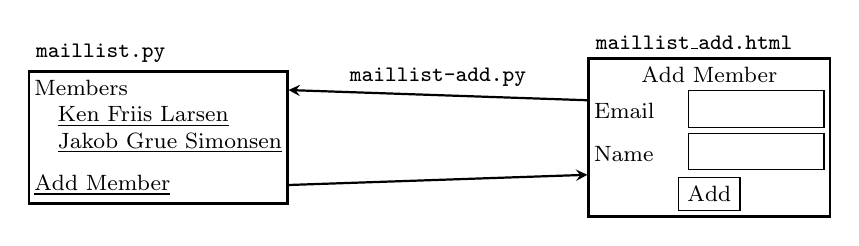
\begin{tikzpicture}[>=stealth]\footnotesize
  \path[inner sep=2pt, thick] 
  (0,0) node[draw] (ML) {%
    \begin{tabular}{@{}l@{}}
      Members \\
      \quad $\underline{\mbox{Ken Friis Larsen}}$\\
      \quad $\underline{\mbox{Jakob Grue Simonsen}}$\\[2mm]
      $\underline{\mbox{Add Member}}$
    \end{tabular}}
  (7,0) node[draw] (ADD) {%
    \begin{tabular}{@{}ll@{}}
      \multicolumn{2}{c}{Add Member}\\
      Email & \fbox{\rule{0mm}{.8em}\hspace{15mm}}\\[.8mm]
      Name & \fbox{\rule{0mm}{.8em}\hspace{15mm}}\\[1mm]
      \multicolumn{2}{c}{\fbox{Add}}
    \end{tabular}};
  \path (ML.north west) node[above right] {\texttt{maillist.py}};
  \path (ADD.north west) node[above right] {\texttt{maillist\_add.html}};
  
  \draw[->,thick] (ML.-20) -- (ADD.197);
  \draw[<-,thick] (ML.20) -- node[above] {\texttt{maillist-add.py}} (ADD.163);
\end{tikzpicture}
\end{center}


% \begin{center}
% \includegraphics[width=\textwidth]{mailing_list_site_map}
% \end{center}

\begin{itemize}
\item The boxes in the diagram represent states where HTML code is displayed
in a browser

\item Unlabelled arrows represent links to a new HTML page, possibly
  generated by a Python script
\item Labelled arrows represent transactions that update the database
  by running a Python script
\end{itemize}
\end{frame}



\begin{frame}[fragile=singleslide]
\frametitle{Example: A Mailing List---Continued} 
\textbf{Step 3: Constructing web forms:} \texttt{maillist\_add.html}:
\begin{small}
\begin{verbatim}
<html><title>Mailing List</title>
  <body>
  <h2>Add Yourself to Mailing List</h2>
  <form action="maillist-add.py" method="post">
  <table>
    <tr><td>Email:<td><input type="text" name="email"></td></tr>
    <tr><td>Name: <td><input type="text" name="name"></td></tr>
    <tr><td colspan="2">
        <input type="submit" value="Add">
    </td></tr>
  </table>  
  </body>
</html>
\end{verbatim}
\end{small}

\textbf{Note:}
\begin{itemize}
\item The file \texttt{maillist-add.py} is the form \emph{action}
\item The form contains two fields called \texttt{email} and \texttt{name}
\end{itemize}
\end{frame}

\begin{frame}[fragile=singleslide]
\frametitle{Example: A Mailing List---Continued}
\textbf{Step 4: Constructing Python files}
\texttt{maillist.py}
\begin{small}
\begin{semiverbatim}
import sqlite3, cgi
try:
    print "Content-type: text/html\(\backslash{}\)n\(\backslash{}\)n"
    db = sqlite3.connect("maillist.db")
    cursor = db.cursor()
    cursor.execute("SELECT email, name FROM Maillist")
    items = cursor.fetchall()
    db.commit()
    lis = "<ul>\(\backslash{}\)n"
    for item in items:
       lis += "<li><a href=\(\backslash{}\)"mailto:%s\(\backslash{}\)">%s.</a></li>" 
              % (item[0], item[1].encode('latin1'))
    lis += "</ul>"
    print makePage("...","""<h1>...</h1>%s
          <p><a href="maillist_add.html">Add Yourself</a></p>
          </body></html>""" % (lis,))
except: 
    cgi.print_exception()
\end{semiverbatim}
\end{small}
\end{frame}

\begin{frame}[fragile=singleslide]
\frametitle{Example: A Mailing List---Continued}

The file \texttt{maillist-add.py}---adding an email address:
\begin{small}
\begin{verbatim}
import sqlite3, cgi
def addEmail(cursor, name, email):
    cursor.execute("""INSERT INTO Maillist (email, name) 
                      VALUES (?, ?)""", (email, name))
def makeDb():
    db = sqlite3.connect("maillist.db")
    return db
try:
    form = cgi.FieldStorage()
    name = form.getfirst('name')   
    email = form.getfirst('email')
    db = makeDb()
    cursor = db.cursor()
    addEmail(cursor, name, email)
    db.commit()
    print "Location: maillist.py\n\n"
except: 
    cgi.print_exception()
\end{verbatim}
\end{small}

\begin{itemize}
\item By sending a \texttt{Location:} header to the browser with location
  \texttt{maillist.py}, information is sent to the browser (via HTTP)
  informing it to request the file \texttt{maillist.py} from the server.
\item As this happens rapidly---and without user interaction---the
  result is that the updated mailing list is displayed for the user.
\item Are there any inconveniences or defects in the scripts above?
\end{itemize}

\end{frame}

% \begin{frame}[fragile=singleslide]
% \frametitle{Factor Out Database Connection}

% By factor out the code to connect to the database to a seperate file,
% say \texttt{mydb.php}, we can include using \texttt{require}, we avoid
% writing password information in all files:
% \begin{small}
% \begin{verbatim}
% <?php
%    // function for establishing connection to the database
%    function mydb_connect() {
%      $dbhost = "mysql.itu.dk"; $user = "kfl";
%      $passwd = "passwd"; $database = "DSDS_E2006";
%      $db = mysql_connect($dbhost, $user, $passwd);
%      if ( $db == 0 ) {
%         die ("Connection to database on '$dbhost' failed");
%      }
%      if ( mysql_select_db($database, $db) == 0 ) {
%         die ("Failed to select database '$database'");
%      }
%      return $db;
%    }
% ?>
% \end{verbatim}
% \end{small}

% % \textbf{Note:} We check the return values from
% % \texttt{mysql\_connect} and \texttt{mysql\_select\_db}
% \end{frame}

% \begin{frame}[fragile=singleslide]
% \frametitle{Extending The Mailing List Example}

% \begin{itemize}
% \item Let us extend our mailing list example so that it is possible to
%   remove names from the list


% \item We consider the four steps again:
%   \begin{itemize}
%   \item \textbf{Step 1:} The data model is unchanged (table \texttt{maillist})

%   \item \textbf{Step 2:} The following data transaction is added:
%     \begin{itemize}
%     \item Deleting an entry from the list

%       \begin{small}
% \begin{verbatim}
% DELETE FROM Maillist WHERE id = 42;
% \end{verbatim}
%       \end{small}
%     \end{itemize}
%   \end{itemize}
% \end{itemize}
% \end{frame}

% \begin{frame}
% \frametitle{Extending The Mailing List Example---Continued}

% \textbf{Step 3:} Constructing a site map:

% % \begin{center}
% % \includegraphics[width=\textwidth]{mailing_list_site_map2}
% % \end{center}
% \begin{center}
% \begin{tikzpicture}[>=stealth]\footnotesize
%   \path[inner sep=2pt, thick] 
%   (0,0) node[draw] (ML) {%
%     \begin{tabular}{@{}ll@{}}
%       Members \\
%       \quad $\underline{\mbox{Ken Friis Larsen}}$&\fbox{Del}\\
%       \quad $\underline{\mbox{Nils Andersen}}$&\fbox{Del}\\[2mm]
%       $\underline{\mbox{Add Yourself}}$
%     \end{tabular}}
%   (7,0) node[draw] (ADD) {%
%     \begin{tabular}{@{}ll@{}}
%       \multicolumn{2}{c}{Add Member}\\
%       Email & \fbox{\rule{0mm}{.8em}\hspace{15mm}}\\[.8mm]
%       Name & \fbox{\rule{0mm}{.8em}\hspace{15mm}}\\[1mm]
%       \multicolumn{2}{c}{\fbox{Add}}
%     \end{tabular}}
%   ;%(3.5, -2) node(DEL){\texttt{maillist2\_del.php}};
%   \path (ML.north west) node[above right] {\texttt{maillist2.php}};
%   \path (ADD.north west) node[above right] {\texttt{maillist2\_add.html}};
  
%   \draw[->,thick] (ML.-14) -- (ADD.197);
%   \draw[<-,thick] (ML.14) -- node[above] {\texttt{maillist2\_add.php}} (ADD.163);
%   \draw[->,thick] (ML.-25) -| (3,-2) node[below] {\texttt{maillist2\_del.php}} -| (ML.south);

% \end{tikzpicture}
% \end{center}




% \begin{itemize}
% \item The file \texttt{maillist2\_del.php} deletes a row from the table
% \item This file expects a form variable \texttt{id}, transferred from
%   \texttt{maillist2.php} as a \texttt{POST} form variable.
% \end{itemize}
% \end{frame}

% \begin{frame}[fragile=singleslide]
% \frametitle{Extending The Mailing List Example---Continued}
% \textbf{Step 4:} Code  PHP files. The file \texttt{maillist2.php}:
% \begin{small}
% \begin{verbatim}
% <html> ...
% <?php 
%   require('mydb.php'); 
%   $db = mydb_connect();
%   // Extract rows from the table
%   $rows = mysql_query("SELECT id, email, name FROM Maillist", $db);
%   // Iterate through the rows
%   while ( $row = mysql_fetch_array($rows) ) {
%     $email = $row['email']; $name = $row['name']; $id = $row['id'];
%     // Display a single row
%     echo '<li>
%           <form action="maillist2_del.php" method="post">
%           <a href="mailto:'.$email.'">'.$name.'</a>
%           <input type="hidden" name="id" value="'.$id.'">
%           <input type="submit" value="Del">
%           </form></li>';
%   }
% ?>
% \end{verbatim}
% \end{small}
% \end{frame}

% \begin{frame}[fragile=singleslide]
% \frametitle{Extending The Mailing List Example---Continued}

% The file \texttt{maillist2\_del.php}:
% \begin{small}
% \begin{verbatim}
% <?php
%   require("mydb.php");       // Include utilities
%   require("formvars.php");

%   $id = $_POST['id'];
%   chk_integer( $id );        // Check form variable

%   $db = mydb_connect();      // Connect to the database

%   // Delete a row
%   mysql_query("DELETE FROM Maillist WHERE id = $id", $db);

%   // Jump to the main page
%   header("Location: maillist2.php");
% ?>
% \end{verbatim}
% \end{small}

% %\textbf{Next time:} We consider among other things how to send email
% %to the email addresses

% \end{frame}

% % \begin{frame}[fragile=singleslide]

% % \frametitle{Generating Unique ID Numbers In MySQL}


% % \begin{itemize}
% % \item In MySQL you can use \texttt{auto\_increment} to generate fresh
% %   ID numbers automatically when inserting new rows into a table:
% %   \begin{small}
% % \begin{verbatim}
% %   CREATE TABLE Users (id int AUTO_INCREMENT PRIMARY KEY,
% %                       name varchar(100) NOT NULL);
% %   INSERT INTO Users (name) VALUES ('Ken Friis Larsen');
% %   INSERT INTO Users (name) VALUES ('Nils Andersen');
% % \end{verbatim}
% %   \end{small}

% %   (Other database systems provide similar functionality)

% % \item In PHP, to get the ID generated for an \texttt{auto\_increment}
% %   column by an \texttt{insert} query, you use the
% %   \texttt{mysql\_insert\_id} function:
% %   \begin{small}
% % \begin{verbatim}
% % <?php 
% %  // Insert a new row
% %  mysql_query("INSERT INTO Users (name) 
% %               VALUES ('Ken Friis Larsen')", $db);

% %  // Get the auto_increment id column
% %  echo "Ken Friis Larsen got ID number ".mysql_insert_id();
% % ?>
% % \end{verbatim}
% %   \end{small}
% % \end{itemize}
% % \end{frame}

% \begin{frame}

% \frametitle{Exercises}

% \begin{itemize}
% \item Constructing a commentary service

% \item Add a functionality allowing the readers of your web pages to
%   comment them\ldots

% \end{itemize}

% \end{frame}

\end{document}



%%% Local Variables: 
%%% mode: latex
%%% TeX-master: t
%%% End: 
